%\documentclass{article}
%\usepackage{graphicx,subfigure}
%\begin{document}

\begin{figure}[!h]
  \centering
  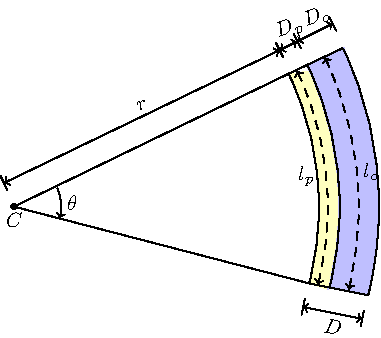
\includegraphics[width=0.9\textwidth]{rmin.pdf}
  \caption{A curved length of fibre with its radius of curvature centred at point $C$. The para cortex is the yellow segment, and its length is shown as the dotted centreline length $l_{p}$. The orthocortex is the blue segment and its length is shown as the dotted centreline length $l_{o}$. The radius of the inner edge of the curved fibre is $r$. The angle subtended at the centre of itsradius of curvature is $\theta$.}
  \label{fig:rmin}
\end{figure}

%\end{document}

